\documentclass[notheorems]{beamer}
\usetheme[secheader]{Lab2C}
%\usetheme{Lab2C} % disable pgf drawing to speed up compilation in development
\usepackage{graphicx}
\usepackage{array}
\usepackage{subcaption}
\usepackage{listings}
\usepackage{color}
\usepackage{algorithmic}
\usepackage{amssymb}
\usepackage[square,sort,comma,numbers]{natbib}
\input{macros.tex}
\DeclareMathOperator{\Bern}{Bern}
\newcommand\independent{\protect\mathpalette{\protect\independenT}{\perp}}
\def\independenT#1#2{\mathrel{\rlap{$#1#2$}\mkern2mu{#1#2}}}

\definecolor{mygray}{rgb}{0.5,0.5,0.5}
\lstset{
numbers=left,
numbersep=5pt,
numberstyle=\tiny\color{mygray}
}

\newif\ifbeamer
\beamertrue
%\setbeamertemplate{footline}[frame number]
%\logo{\includegraphics[height=0.8cm]{ieee_logo.eps}}
\title{My Academic Background, Project Experiences and Research Works}
\author{Feng Zhao\inst{1}}
\institute{\inst{1}Dept. of Electronic Engineering, Tsinghua University, 2017- Present
\and\inst{2}Department of Mathematical Sciences, Tsinghua University, 2013-2017
	\\ \vskip 0.5cm Noah Group Interview 2021}
\date{\today}
\begin{document}
\begin{frame}
	\titlepage
\end{frame}
\begin{frame}{Internship and Teaching Experiences}
\begin{block}{June 2017 - Aug.}
	Research Assistant for Mechanical Simulation Group\\
	\raggedleft\small\textit{CRRC Qingdao Sifang}, Qingdao, China
\end{block}
\begin{block}{July 2019 - Aug.}
	Software Developer for air-conditioner Monitor System\\
	\raggedleft\small\textit{Media}, Shunde, China
\end{block}
\begin{block}{Sept. 2020 - Jan. 2021}
	Teaching Assistant for Machine Learning Course\\
	\raggedleft\small\textit{Tsinghua Berkeley Shenzhen Institute}
\end{block}
\begin{block}{Mar. 2021 - June}
	Teaching Assistant for Probability Theory Course\\
	\raggedleft\small\textit{Tsinghua Berkeley Shenzhen Institute}
\end{block}
\end{frame}
%\section*{Outline}
\begin{frame}
	\tableofcontents
	% the whole story goes
	% as follows:
	% first we need to remove outliers given a community
	% then we need to detect the communities
	% finally using side information we can improve
	% the accuracy of the detection
\end{frame}
\section[Background]{Background of Community Detection}
\begin{frame}{Community Detection}
	\begin{columns}
		\column{0.5\textwidth}
		\begin{figure}
			\includegraphics[width=0.8\textwidth]{cd.png}
		\end{figure}
	\column{0.5\textwidth}
	Community Detection is inferring the group of vertices which are more
	densely connected in a network
	\end{columns}
	\begin{columns}
		\column{0.33\textwidth}
		\begin{figure}
			\includegraphics[width=\textwidth]{benno2t.pdf}
		\end{figure}
		\column{0.05\textwidth}
		$\Rightarrow$
		\column{0.5\textwidth}
		\begin{figure}
		\includegraphics[width=\textwidth]{bennot.pdf}
		\end{figure}
	\end{columns}
\end{frame}
\begin{frame}{Application Domain}
	\begin{columns}[T] % contents are top vertically aligned
		\column{.6\textwidth}
		\begin{figure}
		\includegraphics[height=4cm]{distributed_computing.jpg}
		\caption*{Job allocation in distributed computing}
		\end{figure}
		\column{.4\textwidth}
		\begin{figure}
		\includegraphics[height=4cm]{recommendation_system.png}
		\caption*{User clustering in recommendation system}
		\end{figure}
		\end{columns}
\end{frame}
\begin{frame}{Model and Algorithms}
	% this slide focuses on the methods:
	% how to achieve the goal
	% of community detection
	\begin{block}{Terminology}
		\begin{itemize}
			\item Network: graph $G(V, E)$
			\item Community: subset of $V$
		\end{itemize}		
	\end{block}
	\vskip 0.5cm
	\begin{columns}
		\column{0.5\textwidth}
		Algorithm Design
		\begin{itemize}
			\item Heuristic Algorithms
			\item Optimization-based algorithm
		\end{itemize}
		Empirical Study
		\begin{itemize}
			\item Better accuracy
			\item lower time complexity
		\end{itemize}
		\column{0.5\textwidth}
		Theoretical Model
		\begin{itemize}
			\item Bayesian Network
			\item Stochastic Block Model
		\end{itemize}
		Asymptotic Study
		\begin{itemize}
			\item When $|V|\to \infty$
			\item How some property changes
		\end{itemize}
	\end{columns}
\end{frame}
\begin{frame}{Benchmark Problem and Evaluation Metric}
		\begin{block}{Stochastic block model}
		\begin{itemize}
		\item a probabilistic model to generate random graph
		\item larger probability for the existence of edges within the same community
		\item smaller probability for the existence of edges between different communities
		\end{itemize}
		\end{block}
		\begin{columns}
			\column{0.3\textwidth}
				\begin{figure}
				\includegraphics[width=\textwidth]{sbm.png}
			\end{figure}
		\column{0.7\textwidth}
		\quad$(G,X)\sim \textrm{SBM}(n, k, p, q)$
		\begin{itemize}
			\item $X$: community labels
			\item $n$: the number of nodes
			\item $k$: the number of communities
			\item $p$: probability of connecting within clusters
			\item $q$: probability of connecting across clusters
		\end{itemize}
		\end{columns}
\end{frame}
\section[Info-Clustering]{Outlier Detection in Communities by Info-Clustering}
\begin{frame}
	\tableofcontents[currentsection]
\end{frame}
\begin{frame}{Background}
	\begin{columns}
		\column{5cm}
		\begin{figure}
			\includegraphics[width=\textwidth]{community_outlier.png}
			\caption{The Community Outlier}
		\end{figure}
		\column{5cm}
		Outlier detection is the identification of abnormal data which differs from the majority of the data.
	\end{columns}
\begin{figure}
\includegraphics[width=0.9\textwidth]{mmi.png}
\caption{Multivariate Mutual Information}
\end{figure}
\end{frame}
% \begin{frame}
% 	\frametitle{Related Work}
% \begin{itemize}
% \item graph based clustering method
% 	\begin{enumerate}
% 		\item \citeauthor{de} in \citeyear{de} proposed a hierarchical density estimate method 
% %to do outlier detection
% 		\item \citeauthor{mac} in \citeyear{mac} proposed a minimum average cost clustering method 
% %which shares the same hierarchical clustering structure with info-clustering.
% 		\item \citeauthor{ic} in \citeyear{ic} proposed info-clustering method
% %which is a hierarchical clustering method.
% 	\end{enumerate}
% \item Graph partition algorithm
% \begin{enumerate}
% \item \citeauthor{psp} in \citeyear{psp} proposed an algorithm to compute the principal sequence of partition 
% \item \citeauthor{pmf} in \citeyear{pmf} proposed a parametric algorithm for the same task 
% \end{enumerate}
% \end{itemize}
% Our work
% \begin{itemize}
% \item Info-Detection method
% \item Improved algorithm for principal sequence of partition
% \end{itemize}
% \end{frame}

% \subsection{Info-Clustering}
\begin{frame}
\frametitle{Formulation and Algorithm}
Formulation of Info-Clustering for Weighted Graphs
\begin{enumerate}
\item graph $G(V, E)$
\item mutual information of two nodes: edge weight $w_{ij}$
\item multivariate mutual information (MMI) of a node set $C$
\item the set $C$ with largest MMI other than $V$ is not outliers
\end{enumerate}
\begin{figure}
	\includegraphics[width=0.9\textwidth]{alg_illustration.eps}
	\caption{Hierarchical partition algorithm find outliers}
\end{figure}
\end{frame}


 \begin{frame}{Experiments and Publications}
 \begin{figure}
 	\centering
 	\includegraphics[width=\textwidth]{pic/outlier_boundary_illustration.eps}
 	\caption{Graph is constructed by Gaussian Kernel} \label{fig:boundary}
 \end{figure}

\normalsize Zhao, F., Ma, F., Li, Y., Huang, S.-L., \& Zhang, L.
 (2019, December).
 Info-Detection: An Information-Theoretic Approach to Detect Outlier. In International Conference on Neural Information Processing (pp. 489-496). Springer, Cham.

 \end{frame}




\section[Ising Model]{Community Detection by Ising Model}
\begin{frame}
	\tableofcontents[currentsection]
\end{frame}
\begin{frame}
\frametitle{Phase transition in classical Ising model}
	\begin{columns}
		\column{0.5\textwidth}
		\begin{figure}
			\includegraphics[width=\textwidth]{monte-carlo-ising-6.png}
			\caption*{Magnetization changes with temperature}
		\end{figure}
		\column{0.5\textwidth}
	In statistical physics, Ising model refers to the magnetic spins that can be in one of two states (+1 or -1).
	
	$T_c$: critical temperature.
	
	\end{columns}
\begin{figure}
	\centering
	\begin{subfigure}{0.4\textwidth}
		\includegraphics[width=0.7\textwidth]{Tlarge.pdf}
		\caption{$T>T_c$, random spins}
	\end{subfigure}~
	\begin{subfigure}{0.4\textwidth}
		\includegraphics[width=0.65\textwidth]{Tsmall.pdf}
		\caption{$T<T_c$, spins align}
	\end{subfigure}
\end{figure}
\end{frame}

% \begin{frame}
% \frametitle{Canonical ensemble}
% \begin{columns}
% 	\column{0.5\textwidth}
% The distribution of particles:
% \begin{equation*}
% P(\sigma = \bar{\sigma}) = \frac{1}{Z} \exp(-\beta H(\bar{\sigma}))
% \end{equation*}
% \begin{itemize}
% 	\item $Z$: partition function
% 	\item $\beta$: inverse temperature
% 	\item $H$: Hamiltonian energy
% 	\item $\sigma \in \{\pm 1\}^n$: particle state 
% \end{itemize}
% 	\column{0.5\textwidth}
% 	\begin{tabular}{ccc}
% 		No & Micro state & Macro state ($H$) \\
% 		1 & $\uparrow\uparrow\uparrow$ & -3 \\
% 		2 & $\uparrow\uparrow\downarrow$ & 1 \\
% 		3 & $\uparrow\downarrow\uparrow$ & 1 \\
% 		4 & $\downarrow\uparrow\uparrow$ & 1 \\
% 		5 & $\uparrow\downarrow\downarrow$ & 1 \\
% 6 & $\downarrow\uparrow\downarrow$ & 1 \\
% 7 & $\downarrow\downarrow\uparrow$ & 1 \\
% 8 & $\downarrow\downarrow\downarrow$ & -3 \\
% 	\end{tabular}
% \end{columns}
% \begin{block}{Hamiltonian for Ising model}
% 	Given a graph $G(V, E)$,
% 	\begin{equation*}
% 	H(\sigma) = -\sum_{\{i,j\} \in E(G)} \sigma_i \cdot \sigma_j
% 	\end{equation*}

% \end{block}

% \end{frame}
% \begin{frame}
% \frametitle{Square-lattice Ising model}
% \begin{block}{spontaneous magnetization}
% 	% 磁化强度
% 	$M = \frac{1}{N} \sum_{i=1}^N \sigma_i$: spontaneous magnetization for $N\to \infty$:
% 	\begin{enumerate}
% 		\item $T< T_c$, $M>0$, spontaneous magnetization exists;
% 		\item $T> T_c$, $M=0$, no spontaneous magnetization.
% 	\end{enumerate}
% \end{block}
% \begin{figure}
% 	\centering
% 	\begin{subfigure}{0.45\textwidth}
% 		\includegraphics[width=\textwidth]{square-lattice.png}
% 		\caption{square lattice}
% 	\end{subfigure}~
% 	\begin{subfigure}{0.53\textwidth}
% 		\includegraphics[width=\textwidth]{monte-carlo-ising-6.png}
% 		\caption{Simulation result}
% 	\end{subfigure}
% \end{figure}

% \end{frame}


% \begin{frame}
% \frametitle{Metropolis algorithm}
% \begin{block}{Charateristics}
% \begin{itemize}
% 	\item commonly used to simulate Ising model
% 	\item single-spin-flip dynamics 
% 	\item stochastic method for optimization
% \end{itemize}
% \end{block}
% 	\begin{algorithmic}[1]
% 	\STATE random initialize $\bar{\sigma}$
% 	\STATE randomly choosing a new state $\bar{\sigma}'$ by flipping one spin site
% 	\STATE compute $\Delta H= H(\bar{\sigma}') - H(\bar{\sigma})$
% 	\IF{$\Delta H < 0$}
% 	\STATE $\bar{\sigma} \leftarrow \bar{\sigma}'$
% 	\ELSE
% 	\STATE with probability $\exp(-\beta \Delta H)$ 
% 	such that $\bar{\sigma} \leftarrow -\bar{\sigma}'$ 
% 	\ENDIF
% 	\STATE repeat 2-8 until convergence
% \end{algorithmic}
% \end{frame}

% \begin{frame}{Community Detection with Side Information}
% 	\begin{columns}
% 		\column{0.5\textwidth}
% 	\begin{figure}
% 		\includegraphics[width=0.8\textwidth]{si.png}
% 		\caption{\scriptsize Graph Model with Side Information}
% 	\end{figure}
% 	\column{0.5\textwidth}
% 	Incorporating side information in graph model
% 	can improve the performance of Community Detection
% 	\begin{block}{Objective}
% 		Investigate quantitatively how side information influences
% 		the detection error rate for a specific graph model
% 	\end{block}
% 	\end{columns}
% \end{frame}
% \subsection{Stochastic Block Model}
% \begin{frame}{Binary Symmetric Stochastic Block Model}
% 	\begin{block}{Characteristics}
% 		\begin{itemize}
% 		\item a probabilistic model to generate random graph
% 		\item larger probability for the existence of edges within the same community
% 		\item smaller probability for the existence of edges between different communities
% 		\end{itemize}
% 		\end{block}
% 		\begin{columns}
% 			\column{0.33\textwidth}
% 				\begin{figure}
% 				\includegraphics[width=\textwidth]{sbm.png}
% 			\end{figure}
% 		\column{0.67\textwidth}
% 		\quad$(G,Y)\sim \textrm{SSBM}(n, p, q)$
% 		\begin{itemize}
% 			\item $Y$: community labels
% 			\item $n$: the number of nodes
% 			\item $p$: probability of connecting within clusters
% 			\item $q$: probability of connecting across clusters
% 		\end{itemize}
% 		\end{columns}	
% \end{frame}
% \begin{frame}{Detection Algorithms and Recovery Metrics}
% 	\begin{description}
% 		\item[Observation] random graph $G$, generated by $\textrm{SSBM}(n,p,q)$;
% 		\item[Estimator] $\hat{Y}(G)$, an algorithm to recover node labels $Y$;
% 		\item[Error probability] $P_e=P(\hat{Y} \neq \pm Y)$
% 	\end{description}
	
% 	\begin{block}{Known Results [Abbe-Bandeira-Hall, 2014]}
% 		\begin{itemize}
% 		\item Community labels $Y$ are symmetric: half $+1$, half $-1$;
% 		\item $p = a\frac{ \log n}{n}, q = b \frac{ \log n}{n}$;
% 		$\sqrt{a} - \sqrt{b} > \sqrt{2}$
% 		\item $P_e \to 0$ as $n \to \infty$.
% 		\end{itemize}
% 	\end{block}
% 	\begin{block}{Problem of Error Rate}
% 	 Does $\lim_{n \to \infty}\frac{\log P_e}{\log n}$
% 	 exist ?
% 	\end{block}
% \end{frame}
% \subsection{Related Works}
% \begin{frame}{Related Works}
% 	% must mention the work of concurrent submission and explain
% 	% the difference between the two
% 	\begin{enumerate}
% 		\item Phase transition study on SBM with side information
% 		[Saad-Nosratinia, 2018]
% 		\item Efficient SDP algorithm to achieve exact recovery
% 		[Sima-Feng, concurrent submission]
% 		\item Weak recovery error rate in SBM
% 		[Zahng-Zhou, 2016]
% 	\end{enumerate}
% 	\begin{block}{This Work}
% 		\begin{enumerate}
% 			\item Optimal error rate study
% 			\item Does not take implementation of algorithm into consideration
% 			\item Strong recovery scenario with side information
% 		\end{enumerate}
% 	\end{block}
% \end{frame}
% \begin{frame}
% 	\frametitle{Phase transition of SBM}
% 	\begin{block}{Exact Recovery of SBM [1]}
% 		$P_e=P(\hat{X} \neq \pm X)$: exact recovery for $n \to \infty$
% 		\begin{enumerate}
% 			\item $\sqrt{a} - \sqrt{b} > \sqrt{2}$, $P_e \to 0$, there exists algorithms to achieve exact recovery;
% 			\item $\sqrt{a} - \sqrt{b} < \sqrt{2}$, $P_e \to 1$, no algorithm can achieve exact recovery
% 		\end{enumerate}
% 	\end{block}
% 	{\scriptsize [1]
% 	Abbe, Emmanuel, Afonso S. Bandeira, and Georgina Hall. "Exact recovery in the stochastic block model." IEEE Transactions on Information Theory 62.1 (2015): 471-487.
% 	}
% 	\end{frame}
	
% 	\section{Stochastic Ising block model}

\begin{frame}
	\frametitle{\large Stochastic Ising block model and its phase transition property}
\begin{itemize}
	\item The Ising model is defined on top of graph generated by SBM.
 	\begin{equation*}
 	P_{\sigma | G} = \frac{1}{Z} \exp(-\beta H(\bar{\sigma}))
 	\end{equation*}
	 \item The studied property: $P_e= \displaystyle\min_{\hat{X}} P(\hat{X} \neq X)$
	 \item $\beta > \beta^*$, $P_e \to 0$, there exists algorithms to achieve exact recovery;
	\item $\beta < \beta^*$, $P_e \to 1$, no algorithm can achieve exact recovery
\end{itemize}
\begin{block}{Metropolis Algorithm}
 \begin{itemize}
 	\item commonly used to simulate Ising model
 	\item single-spin-flip dynamics
 	\item stochastic method for optimization
 \end{itemize}
\end{block}
% 	\item The Hamiltonian energy is compensated by repelling interaction between nodes without edge connection
% 	\begin{equation*}
% 	H(\sigma) = \frac{p+q}{2}\sum_{\{i,j\} \not\in E(G)} \sigma_i \cdot \sigma_j - \sum_{\{i,j\} \in E(G)} \sigma_i \cdot \sigma_j
% 	\end{equation*}
% 	\end{itemize}
% 	\begin{description}
% 		\item[Observation] random graph $G$, generated by $\textrm{SBM}(n,p,q)$;
% 		\item[Estimator] $\hat{X}^*$, generated by SIBM
% 		\item[Error Probability] $P_e=P(\hat{X} \neq \pm X) = ?$
% 	\end{description}
	\end{frame}
	
% 	\begin{frame}
% 	\frametitle{Phase transition of SIBM}
% 	\begin{block}{Assumptions}
% 		\begin{itemize}
% 			\item Community labels $X$ are symmetric: half $+1$, half $-1$;
% 			\item $p = a\frac{ \log n}{n}, q = b \frac{ \log n}{n}$;
% 			\item $n \to \infty$.
% 		\end{itemize}
% 	\end{block}
% 	\begin{block}{Exact Recovery of SBM by $\hat{X}^*$}
% 		$P_e=P(\hat{X} \neq \pm X)$: exact recovery for $n \to \infty$
% 	\begin{enumerate}
% 		\item $\beta > \beta^*$, $P_e \to 0$, there exists algorithms to achieve exact recovery;
% 		\item $\beta < \beta^*$, $P_e \to 1$, no algorithm can achieve exact recovery
% 	\end{enumerate}
% 	where
% 	\begin{equation*}
% 	\beta^* = \frac{1}{2} \log \frac{a+b-2 - \sqrt{(a+b-2)^2-4ab}}{2b}
% 	\end{equation*}
% 	\end{block}
	
% 	\end{frame}
	
	\begin{frame}
	\frametitle{Simulation results and publication}
	Metropolis algorithm is used to approximate $\hat{X}^*$
	
% add \href{run:./OrbiteEul.mp4}{OrbiteEul.mp4} to invoke the
% local mp4 file
	\begin{figure}
		\centering
		\begin{subfigure}{0.45\textwidth}
			\includegraphics[width=\textwidth]{000.png}
			\caption{\href{run:./demo.mp4}{Initial} label for $\textrm{SBM}(300, 16, 4)$}
		\end{subfigure}~
		\begin{subfigure}{0.53\textwidth}
			\includegraphics[width=\textwidth]{beta_trans-2020-11-28.eps}
			\caption{$\textrm{SBM}(9000, 16, 4), \beta^*=0.198$}
		\end{subfigure}
	\end{figure}
	Zhao, F., Ye, M., Huang, S.-L. Exact Recovery of Stochastic Block Model by Ising Model. Entropy 2021, 23, 65.
	
\end{frame}
	
	
	
% 	%\section{Conclusion}
% 	\begin{frame}
% 	\frametitle{Conclusion}
% 	On-going work:
% 	\begin{itemize}
% 	\item Extension of SIBM to multiple community case;
% 	\item connection with other community detection method is explored
% 	\end{itemize}
% 	\begin{figure}
% 		\includegraphics[width=0.8\textwidth]{overview.pdf}
% 		\caption{Connection between different parts}
% 	\end{figure}
% 	\end{frame}
\section[Side Information]{Community Detection with Side Information}
\begin{frame}
	\tableofcontents[currentsection]
\end{frame}
\begin{frame}{Background}
	\begin{columns}
		\column{0.5\textwidth}
	\begin{figure}
		\includegraphics[width=0.8\textwidth]{si.png}
		\caption{\scriptsize Graph Model with Side Information}
	\end{figure}
	\column{0.5\textwidth}
	Incorporating side information in graph model
	can improve the performance of Community Detection
	\begin{block}{Objective}
		Investigate quantitatively how side information influences
		the detection error rate for SBM
	\end{block}
	\end{columns}
	\begin{block}{Known Results [Abbe-Bandeira-Hall, 2014]}
		\begin{itemize}
		\item Community labels $X$ are symmetric: half $+1$, half $-1$;
		\item $p = a\frac{ \log n}{n}, q = b \frac{ \log n}{n}$;
		$\sqrt{a} - \sqrt{b} > \sqrt{2}$
		\item $P_e \to 0$ as $n \to \infty$.
		\end{itemize}
	\end{block}
\end{frame}

\begin{frame}
\frametitle{Binary Symmetric SBM with Side Information}
\begin{block}{Characteristics}
\begin{itemize}
	\item   Each node includes $m$ additional observations with
	finite-cardinality alphabet.
	%\begin{equation*}
%		x_{i1}, x_{i2}, \dots, x_{im} \in \{1, 2, \dots, |\mathcal{X}|\}
%	\end{equation*}
	\item The extra observations at each node are sampled from distribution $p_0$
	or $p_1$ depending on the node label.
	\item Given the node label, side information are conditionally independent of the random
	graph $G$.
\end{itemize}
\end{block}
Rényi divergence with order $\frac{1}{2}$:
\begin{equation*}
	D_{1/2}(p_0 || p_1) = -2\log(\sum_{x \in \mathcal{X}} \sqrt{p_0(x)p_1(x)} )
\end{equation*}
\end{frame}

% \begin{frame}\frametitle{Exact Recovery Error Rate}
% \begin{block}{Maximum Likelihood}
% \begin{itemize}
% 	\item Theoretically optimal recovery method
% 	\begin{align*}
% 		\hat{Y} &= \arg\max_y\ \Pr(x,G|Y=y) \notag \\
% 		\textrm{s.t.} \ & y_i \in \{\pm 1\}, \sum_{i=1}^n y_i=0 \label{eq:mle}
% 	\end{align*}
% 	\item Achieves the optimal error rate $P_e=P(\hat{Y} \neq Y)$
% \end{itemize}
% \end{block}
% Recall: Rényi divergence with order $\frac{1}{2}$:
% \begin{equation*}
% 	D_{1/2}(p_0 || p_1) = -2\log(\sum_{x \in \mathcal{X}} \sqrt{p_0(x)p_1(x)} )
% \end{equation*}
% \end{frame}
% \section{Main Results}
\begin{frame}{Optimal Error Rate for SBM with Side Information}
\begin{enumerate}
	\item Dense Case: $\gamma=\frac{m}{n}, p, q$ are constants
		\begin{equation*}
		-\lim_{n\to \infty} \frac{1}{n}\log P_e =  \gamma D_{1/2}(p_0 || p_1) + D_{1/2}(\Bern(p)||\Bern(q))
		\end{equation*}
	\item Sparse Case: $\gamma=\frac{m}{ \log n},
	a=\frac{np}{\log n}, b=\frac{nq}{\log n}$ are constants
		\begin{equation*}\label{eq:PeMainL}
		-\lim_{n\to \infty}\frac{\log P_e}{\log n}=\gamma D_{1/2}(p_0||p_1) + (\sqrt{a} - \sqrt{b})^2-2
		\end{equation*}
		as long as
		\begin{align*}
			(\sqrt{a}-\sqrt{b})^2-2 
			> 3a^{1/3}b^{1/3}(a^{1/6}-b^{1/6})^2\label{eq:oneC}
		\end{align*}	
\end{enumerate}
Zhao, F., Sima, J., Huang, S.-L. On the Optimal Error Rate of Stochastic Block Model with Symmetric Side Information.
ITW 2021
\end{frame}
% \begin{frame}
% \frametitle{Discussion of Main Results}
% \begin{enumerate}
% 	\item SBM with no side information: $\gamma = 0$, $P_e$ decays like $n^{2-(\sqrt{a} - \sqrt{b})^2}$
% 	\item Connection with Hypothesis Testing Problem and Gärtner Ellis Theorem
% 	\item Can we remove the additional condition?
% 	$(\sqrt{a}-\sqrt{b})^2-2 
% 	> 3a^{1/3}b^{1/3}(a^{1/6}-b^{1/6})^2$
% 	% This condition is used to control the error
% 	% of two pairs is smaller than that of one pair in order.
% 	\item Main results different from the phase transition solution,
% 	which is the Chernoff information
% 	between $\textrm{Pois}(\frac{a}{2},\frac{b}{2})\times P_0$ and $\textrm{Pois}(\frac{b}{2}, \frac{a}{2})\times P_1$
% 	[Asadi-Abbe-Verdú,2017]
% \end{enumerate}

% \end{frame}
% %\section{Sketch of Proof}

% \section{Conclusion}
% \begin{frame}
% \frametitle{Conclusion}
% \begin{itemize}
% \item The detection error can be
% characterized by Rényi divergence and the parameters of SBM
% \item Our result provides insight on the
% number of features and nodes needed for community
% detection task.
% \end{itemize}
% \end{frame}
\section{Other Works}
\begin{frame}
	\tableofcontents[currentsection]
\end{frame}
\subsection{Universally Good Activation Function}
\begin{frame}
	\frametitle{\small On the Universally Good Activation Function for One Node Neural Network}
	\begin{columns}
	\column{0.5\textwidth}
	\begin{figure}
	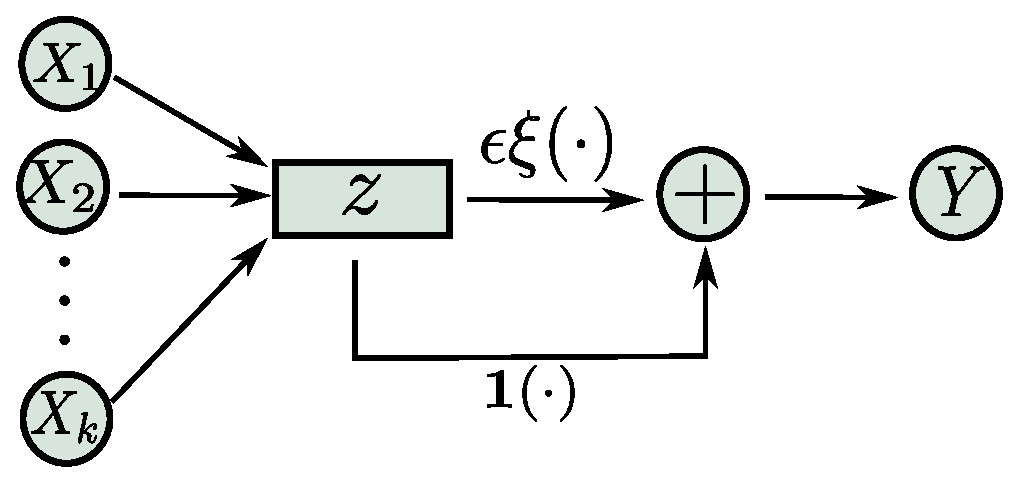
\includegraphics[width=\textwidth]{./network_structure.eps}
	\end{figure}
	\column{0.5\textwidth}
	\begin{itemize}
		\item $X,Y$ are independent
		\item  $\epsilon$ is small
		\item find $\sigma(z) = z + \epsilon \xi(z)$ to minimize the error $E(\sigma)$
	\end{itemize}
	$$
	E(\sigma)= \mathbb{E}[\min_{w} || Y - \sigma(X w) ||^2]
	$$
	\end{columns}
	\begin{theorem}
		Suppose $\xi(z)$ is a polynomial no more than $m$-order and $m\ll k$, then the optimal $\xi$ is $\xi_m(z) = \frac{1}{\sqrt{m! n}}H_m(\frac{n}{\sqrt{k}} z)$ and the optimal value is
		$$
		E(\sigma) = 1-\frac{k}{n}  - (1-\frac{k}{n})(m-1)  \epsilon^2 + o(\epsilon^2)
		$$
		\end{theorem}
\end{frame}
\subsection{Temporal Cooperation Efficiency in Wireless Networks}
\begin{frame}{\large On the Temporal Cooperation Efficiency in Wireless Networks}
	\begin{columns}
		\column{0.5\textwidth}
		\begin{figure}
			\def\svgwidth{\textwidth}
			\input{geometric_interpretation_v2.eps_tex}
			\caption{One agent locating itself with information from anchors and previous time steps}
			\label{f1}
		\end{figure}
		\column{0.5\textwidth}
		\begin{itemize}
			\item Unbiased position estimator $\hat{\bm{P}}$
			\item Study the lower bound of localization error by Cramér-Rao
			\item The lower bound decays exponentially
			with the number of previous positions $N$ used
		\end{itemize}
		$$
		\min_{\hat{\bm{P}}} \mathbb{E}[|| \hat{\bm{P}} - \bm{P} ||^2]
		\leq \frac{1}{\lambda^{N}}
		$$
	\hspace{0.8cm}	for some $\lambda > 1$.
	\end{columns}

\end{frame}

\begin{frame}
	\frametitle{}
	\begin{block}{}
	\centering
	{\Huge Questions and Answers}
	\end{block}
\end{frame}

\end{document}
